%!TEX root = ../these.tex

\section{Основные понятия}

Проектирование управляющих программ
для технологического оборудования термической резки ---
это сложный, многоступенчатый процесс,
в котором можно выделить по крайней мере следующие этапы:
\begin{enumerate}
  \item
  Геометрическое моделирование и кодирование
  геометрии деталей / заготовок
  \item
  Разработка раскройной карты листового материала,
  \item
  Проектирование маршрута движения режущего инструмента
  по раскройной карте
  с учетом технологических ограничений оборудования
  \item
  Собственно генерирование управляющей программы
  для конкретного вида станка с ЧПУ
\end{enumerate}

Хотя вопросы, связанные с разработкой раскройной карты
\cite{bi:Nesting}
(или говоря кратко --- раскроем),
находятся вне темы данной диссертационной работы,
тем не менее,
невозможно не упомянуть
значительный вклад советских и российских исследователей
в теорию оптимизации раскроя.
Работы в этой предметной области
были начаты выдающимися учёными В.А.~Залгаллером
и Л.В.~Канторовичем
\cite{bi:Nesting0}
и продолжены в уфимской научной школе
Э.А.~Мухачевой и ее учениками:
А.Ф.~Валеевой,
М.А.~Верхотуровым,
В.М.~Картаком,
В.В.~Мартыновым,
А.С.~Филипповой, и др.
\cite{bi:мухачева1984,bi:мухачева1998}

\begin{figure}
  \centering
  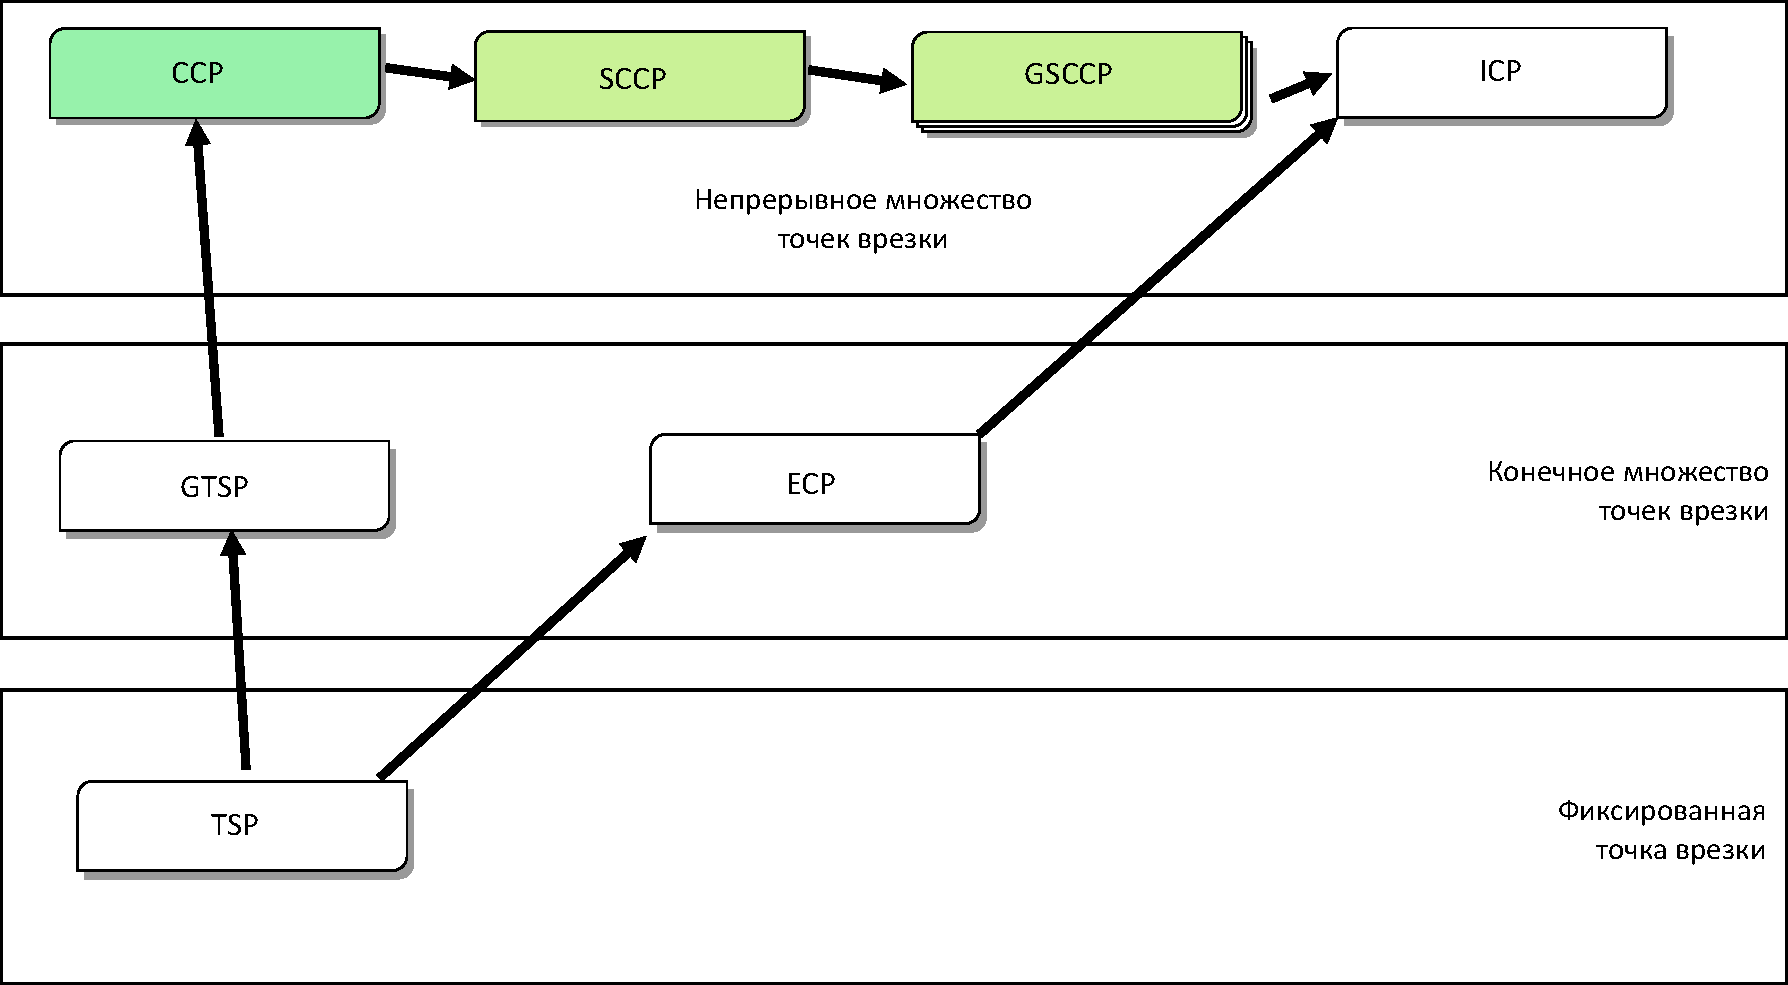
\includegraphics[width=0.95\textwidth]{classes.pdf}
  \caption{Классификация задач резки}
  \label{fig:cut-classes}
\end{figure}
